\documentclass[12pt,a4paper]{article}
\usepackage{../.tex/mcs-notes}
\usepackage{todonotes}
\usepackage{multicol}
% \usepackage{inkscape}
\usepackage{float}
\usepackage[all]{xy}
\CompileMatrices

\settitle
{Геометрия и топология.}
{Евгений Анатольевич Фоминых}
{differential-geometry/main.pdf}
\date{}

\newcommand{\const}{\ensuremath{\mathrm{const}}\xspace}
\newcommand{\Id}{\ensuremath{\mathrm{Id}}\xspace}
\newcommand{\Ker}{\ensuremath{\mathrm{Ker}}\xspace}
\newcommand{\Img}{\ensuremath{\mathrm{Im}}\xspace}
\newcommand{\diam}{\ensuremath{\mathrm{diam}}\xspace}
\newcommand{\Int}{\ensuremath{\mathrm{Int}}\xspace}
\newcommand{\Ext}{\ensuremath{\mathrm{Ext}}\xspace}
\newcommand{\Cl}{\ensuremath{\mathrm{Cl}}\xspace}
\newcommand{\Fr}{\ensuremath{\mathrm{Fr}}\xspace}
\newcommand{\SCl}{\ensuremath{\mathrm{SCl}}\xspace}
\newcommand{\Lin}{\ensuremath{\mathrm{Lin}}\xspace}
\newcommand{\Homeo}{\ensuremath{\mathrm{Homeo}}\xspace}
\newcommand{\Aff}{\ensuremath{\mathrm{Aff}}\xspace}
\newcommand{\Iso}{\ensuremath{\mathrm{Iso}}\xspace}
\renewcommand{\Pr}{\ensuremath{\mathrm{Pr}}\xspace}
\newcommand{\conv}{\ensuremath{\mathrm{conv}}\xspace}
\newcommand{\RelInt}{\ensuremath{\mathrm{RelInt}}\xspace}
\DeclareMathOperator*{\bigtimes}{\text{\raisebox{-6pt}{\scalebox{3}{$\times$}}}}
\newcommand{\FAC}{\ensuremath{\mathrm{FAC}}\xspace}
\newcommand{\SAC}{\ensuremath{\mathrm{SAC}}\xspace}
\newcommand{\T}{\ensuremath{\mathrm{T}}\xspace}
\newcommand{\ex}{\ensuremath{\mathrm{ex}}\xspace}
\newcommand{\ind}{\ensuremath{\mathrm{ind}}\xspace}
\newcommand{\incl}{\mathrm{in}}
\newcommand{\sk}{\mathrm{sk}}

\begin{document}
    \maketitle

    \listoftodos[TODOs]

    \tableofcontents

    \vspace{2em}

    Литература:
    \begin{itemize}
        \item Виро О.Я., Иванов О.А., Нецветаев Н.Ю., Харламов В.М., ``Элементарная топология'', М.:МЦНМО, 2012.
        \item James Munkres, ``Topology''.
    \end{itemize}

    \section{Алгебраическая топология}

    \subsection{Фундаментальная группа}

    \begin{definition}
        \emph{Ретракция} --- непрерывное отображение $f: X \to A$, где $A$ --- подпространство $X$, что $f|_A = \Id_A$.

        Если существует ретракция $f: X \to A$, то $A$ называется \emph{ретрактом} пространства $X$.
    \end{definition}

    \begin{example}\ 
        \begin{enumerate}
            \item Всякое одноточечное подмножество является ретрактом.
            \item Никакое двухточечное подмножество прямой не является ретрактом.
        \end{enumerate}
    \end{example}

    \begin{theorem}
        Пусть дано подпространство $A$ пространства $X$. TFAE
        \begin{enumerate}
            \item $A$ --- ретракт $X$.
            \item всякое непрерывное отображение $g: A \to Y$ продолжается до непрерывного отображения $X \to Y$.
        \end{enumerate}
    \end{theorem}

    \begin{proof}
        Пусть $A$ --- ретракт. Тогда есть ретракция $\rho: X \to A$, а значит $g \circ \rho$ --- продолжение $g$ на $X$.

        С другой стороны, если всякое непрерывное $g: A \to Y$ продолжимо до непрерывного $X \to Y$, то ретракцию $A$ можно получить как продолжение $\Id_A: A \to A$.
    \end{proof}

    \begin{lemma}\label{retraction-lemma}
        Пусть дано подпространство $A$ пространства $X$ и точка $x \in A$. Если $\rho: X \to A$ --- ретракция, а $\incl: A \to X$ --- включение (тождественное отображение), то $\rho_\star: \pi_1(X, x) \to \pi_1(A, x)$ --- сюръекция, а $\incl_\star: \pi_1(A, x) \to \pi_1(X, x)$ --- инъекция.
    \end{lemma}

    \begin{proof}
        $\rho \circ \incl = \Id_A$. Следовательно $(\rho \circ \incl)_\star = \rho_\star \circ \incl_\star = \Id_\star = \Id$, откуда следует, что $\rho_\star$ --- сюръекция, а $\incl_\star$ --- инъекция.
    \end{proof}

    \begin{theorem}[Борсука]
        Не существует ретракции $D^n \to S^{n-1}$.
    \end{theorem}

    \begin{proof}[Доказательство в размерности 2]
        Предположим противное. Пусть $\rho: D^2 \to S^1$ --- ретракция, $x \in S^1$. Из леммы \ref{retraction-lemma} следует, что $in_*: \pi_1(S^1) \to \pi_1(D^2)$ должно быть инъекцией. Но $\pi_1(S^1) = \ZZ$, а $\pi_1(D^2) = \{0\}$. А инъекции $\ZZ \to \{0\}$ не существует --- противоречие.
    \end{proof}

    \begin{remark}
        На самом деле рассуждение работает в любой размерности. Только вместо $\pi_1$ надо взять $\pi_{n-1}$. Там опять же окажется, что лемма верна, $\pi_{n-1}(D^n)$ тривиальна, а $\pi_{n-1}(S^{n-1})$ --- содержит $\ZZ$ как подгруппу.
    \end{remark}

    \begin{definition}
        Точка $a \in X$ называется \emph{неподвижной точкой} отображения $f: X \to X$, если $f(a) = a$.

        Пространство $X$, говорят, \emph{обладает свойством неподвижной точки}, если всякое непрерывное отображение $f: X \to X$ имеет неподвижную точку.
    \end{definition}

    \begin{example}
        $[a; b]$ обладает свойством неподвижной точки.
    \end{example}

    \begin{theorem}[Брауэра]
        Любое непрерывное отображение $f: D^n \to D^n$ имеет неподвижную точку.
    \end{theorem}

    \begin{proof}[Доказательство в размерности 2]
        Предположим противное, $f(x) \neq x$ для всех $x \in D^2$. Построим $g: D^2 \to S^1$ как пересечение открытого луча $(f(x); x; \infty)$ и $S^1$. Несложно удостовериться, что для всех точек $x$, что $f(x) \neq x$, функция $g$ определена и непрерывна в некоторой окрестности $x$. Это противоречит теореме Борсука.
    \end{proof}

    \begin{remark}
        В точности также это можно доказать для любой размерности, но потребуется теорема Борсука большей размерности.
    \end{remark}

    \begin{definition}
        $X$ и $Y$ называются \emph{гомотопически эквивалентными} (и пишут $X \sim Y$), если существуют непрерывные отображения $f: X \to Y$ и $g: Y \to X$ такие, что $g \circ f \sim \Id_X$ и $f \circ g \sim \Id_Y$.

        Такие $f$ и $g$ называются \emph{гомотопически обратными} отображениями. При этом каждое из них называется \emph{гомотопической эквивалентностью}.
    \end{definition}

    \begin{example}
        $\RR^n$ гомотопически эквивалентно $\{0\}$.
    \end{example}

    \begin{definition}
        Ретракция $f: X \to A$ называется \emph{деформационной ретракцией}, если её композиция с включением $\incl: A \to X$ гомотопна тождественному отображению, т.е.
        \[\incl \circ f \sim \Id_X.\]

        Если существует деформационная ретракция $X$ на $A$, то $A$ называется \emph{деформационным ретрактом} пространства $X$.
    \end{definition}

    \begin{theorem}
        Деформационная ретракция --- гомотопическая эквивалентность.
    \end{theorem}

    \begin{proof}
        Действительно, если $f: X \to A$ --- деформационная ретракция, а $\incl: A \to X$ включение, то $f \circ \incl = \Id_A \sim \Id_A$ и
        \[\incl \circ f \sim \Id_A\]
        по оперделению деформационной ретракции. Следовательно $f$ и $\incl$ --- гомтопически обратные друг другу деформационные ретракции.
    \end{proof}

    \begin{corollary}
        Деформационные ретракты гомотопически эквивалентны своим исходным пространствам.
    \end{corollary}

    \begin{example}\ 
        \begin{enumerate}
            \item $S^{n-1}$ --- деформационный ретракт $\RR^n \setminus \{0\}$.
            \item $S^1$ --- деформационный ретракт ленты Мёбиуса и кольца ($S^1 \times [0; 1]$).
            \item Букет $n$ окружностей и окружность с $n$ радиусами --- деформационный ретракт плоскости без $n$ точек.
            \item Букет двух окружностей --- деформационный ретракт тора с дыркой.
        \end{enumerate}
    \end{example}

    \begin{theorem}
        Гомотопическая эквивалентность --- ``отношение эквивалентности'' между топологическими пространствами.
    \end{theorem}

    \begin{proof}
        \begin{itemize}
            \item \textbf{Рефлексивность.} Очевидна, так как $\Id$ является деформационным ретрактом $X \to X$.
            \item \textbf{Симметричность.} Если $X \sim Y$, то есть $f: X \to Y$ и $g: Y \to X$, что $g \circ f \sim \Id_X$ и $f \circ g \sim \Id_Y$. Тогда $Y \sim X$.
            \item \textbf{Транзитивность.} Пусть $X \sim Y \sim Z$. Тогда имеются $f: X \to Y$, $g: Y \to X$, $h: Y \to Z$ и $i: Z \to Y$, что $g \circ f \sim \Id_X$, $f \circ g \sim \Id_Y$, $i \circ h \sim \Id_Y$, $h \circ i \sim \Id_Z$. Следовательно
                \[
                    (g \circ i) \circ (h \circ f)
                    = g \circ (i \circ h) \circ f
                    \sim g \circ \Id_Y \circ f
                    = g \circ f
                    \sim \Id_X
                \]
                и
                \[
                    (h \circ f) \circ (g \circ i)
                    = h \circ (f \circ g) \circ i
                    \sim h \circ \Id_Y \circ i
                    = h \circ i
                    \sim \Id_Z.
                \]
                Следовательно $(h \circ f)$ и $(g \circ i)$ --- гомотопически обратные гомотопические эквивалентности. Значит $X \sim Z$.
        \end{itemize}
    \end{proof}

    \begin{definition}
        Класс пространств, гомотопически эквивалентных данному $X$, называется \emph{гомотопическим типом}. Свойства (характеристики) топологических пространств, одинаковые у гомотопически эквивалентных, --- \emph{гомотопические свойства} (\emph{гомотопические инварианты}).
    \end{definition}

    \begin{exercise}
        Число компонент (линейной) связности --- гомотопический инвариант.
    \end{exercise}

    \begin{theorem}
        Пусть $X$ и $Y$ --- гомотопно эквивалентные поверхности, а $f: X \to Y$, $g: Y \to X$ --- гомотопически обратные гомотопические эквивалентности. Пусть также фиксирована $x_0 \in X$. Тогда
        \[\pi_1(X, x_0) \simeq \pi_1(Y, f(x_0)).\]
    \end{theorem}

    \begin{proof}
        \begin{thlemma}
            Пусть $f, g: X \to Y$ --- непрерывные отображения, а $H: X \times [0; 1] \to Y$ --- гомотопия между $f$ и $g$. Пусть также даны $x_0 \in X$, $y_0 := f(x_0)$, $y_1 := g(x_0)$ и путь $\gamma(t) := H(x_0, t)$ из $y_0$ в $y_1$. Обозначим за $T_\gamma$ --- сопряжение по пути $\gamma$, т.е. $T_\gamma(\alpha) = \gamma^{-1} \alpha \gamma$. Тогда
            \[f_\star = T_\gamma \circ g_\star.\]
        \end{thlemma}

        \begin{proof}
            Условие равенства функций $f_\star = T_\gamma \circ g_\star$ означает, что для всякого $\alpha \in \Omega(X, x_0)$
            \[f_\star([\alpha]) = T_\gamma(g_\star([\alpha])).\]
            Последнее значит, что
            \[[f \circ \alpha] = [\gamma^{-1} (g \circ \alpha) \gamma],\]
            или говоря иначе,
            \[f \circ \alpha \sim \gamma^{-1} (g \circ \alpha) \gamma.\]
            При этом заметим, что
            \[f \circ \alpha = H(\alpha(s), 0), \qquad g \circ \alpha = H(\alpha(s), 1).\]

            Рассмотрим
            \[F: [0; 1]^2 \to X \times [0; 1], (s, t) \mapsto (\alpha(s), t).\]
            Несложно видеть, что
            \[
                F(s, 0) = (\alpha(s), 0),
                \qquad
                F(s, 1) = (\alpha(s), 1),
                \qquad
                F(0, t) = F(1, t) = (x_0, t).
            \]
            Таким образом
            \[
                (H \circ F)(s, 0) = f \circ \alpha,
                \qquad
                (H \circ F)(s, 1) = g \circ \alpha,
                \qquad
                (H \circ F)(0, t) = F(1, t) = \gamma.
            \]
            
            Зафиксируем в $[0; 1]^2$ линейные пути $\varphi: (0, 0) \mapsto (1, 0)$ и $\psi: (0, 0) \mapsto (0, 1) \mapsto (1, 1) \mapsto (1, 0)$. Несложно видеть, что
            \[H \circ F \circ \varphi = f \circ \alpha, \qquad H \circ F \circ \psi = \gamma^{-1} (g \circ \alpha) \gamma.\]
            При этом $[0; 1]^2$ выпукло, значит есть гомотопия $G$, переводящая $\varphi$ в $\gamma$. В таком случае $H \circ F \circ G$ --- гомотопия, переводящая $f \circ \alpha$ в $\gamma^{-1} (g \circ \alpha) \gamma$.
        \end{proof}

        Заметим, что $g \circ f$ гомотопно $\Id_X$. Значит в контексте $x_0$ и $\pi_1(X, x_0)$ есть некоторое сопряжение $T_\gamma$, что
        \[T_\gamma \circ (g \circ f)_\star = (\Id_X)_\star = \Id.\]
        При этом $T_\gamma$ есть изоморфизм групп (биекция). Это в частности означает, что $g_\star \circ f_\star$ является биекцией. Отсюда следует, что $g_\star$ инъективно, а $f_\star$ сюръективно.

        Повторяя рассуждения в обратную сторону, получаем, что $f_\star$ и $g_\star$ являются биекциями. Поэтому
        \[\pi_1(X, x_0) \simeq \pi_1(Y, f(x_0)).\]
    \end{proof}

    \begin{corollary}
        $f_\star$ (кроме того, что индуцирует биекцию из множеств компонент линейной связности $X$ и их фундаментальных групп в множества тех же у $Y$) индуцирует изоморфизмы фундаментальных групп компонент линейной связности $X$.
    \end{corollary}

    \begin{corollary}
        Если $X$ линейно связно (а тогда $Y$ тоже), то $\pi_1(X) \simeq \pi_1(Y)$.
    \end{corollary}

    \begin{definition}
        Топологическое пространство $X$ \emph{стягиваемо}, если гомотопически эквивалентно точке.
    \end{definition}

    \begin{lemma}
        TFAE
        \begin{enumerate}
            \item $X$ стягиваемо.
            \item $\Id_X$ гомотопно константному отображению.
            \item Некоторая точка --- деформационный ретракт.
            \item Всякая точка --- деформационный ретракт.
        \end{enumerate}
    \end{lemma}

    \begin{example}
        Например, стягиваемы следующие пространства.
        \begin{enumerate}
            \item $\RR^n$.
            \item Выпуклые множества.
            \item Звёздные множества.
            \item Деревья.
        \end{enumerate}
    \end{example}

    \begin{lemma}
        Пусть $h: S^1 \to X$ --- непрерывное отображение. TFAE
        \begin{enumerate}
            \item $h$ гомотопно постоянному отображению.
            \item $h$ продолжается до непрерывного отображения $D^2 \to X$.
            \item $h_\star$ --- тривиальный гомоморфизм.
        \end{enumerate}
    \end{lemma}

    \begin{proof}
        \begin{itemize}
            \item[$1 \Rightarrow 2$)] Существует гомотопия $H$ между $h$ и константным отображением. Это значит, что $H: S^1 \times [0; 1] \to X$ --- непрерывно, и $H(x, 1) = \const$. Это значит, что пространство $S^1 \times [0; 1]$ можно склеить по множеству $S^1 \times \{1\}$ (так как на нём $H$ константна) и $H$ переопределится в некоторую функцию $H'$. При этом множество-прообраз $H'$ гомеоморфно $D^2$. Следовательно можно считать, что $H': D^2 \to X$. При этом $H'$ является доопределением, так как $H'|_{S^1} = H|_{S^1 \times \{0\}} = h$.
            \item[$2 \Rightarrow 1$)] Пусть $h$ продолжена до $H$ на $D^2$. Тогда определим
                \[G: S^1 \times [0; 1] \to X, (\alpha, r) \mapsto H(r e^{\alpha i}).\]
                Несложно видеть, что $G$ --- гомотопия между $h$ и константным отображением.
            \item[$1 \Leftrightarrow 3$)] Если $h_\star$ является тривиальным гомоморфизмом фундаментальных групп, то $h = h \circ \alpha \sim \const$, где $\alpha$ --- один оборот по окружности, т.е. $h$ гомотопно константному отображению.

                Если $h$ гомотопно постоянному отображению, то $\alpha \circ h = h \sim \const$, т.е. $f_\star([\alpha]) = e$. При этом $[\alpha]$ порождает группу $\pi_1(S^1)$. Следовательно, $h_\star$ --- тривиальный гомоморфизм.
        \end{itemize}
    \end{proof}

    \begin{theorem}[основная теорема алгебры]
        Всякий многочлен из $\CC[z]$ положительной степени имеет корень.
    \end{theorem}

    \begin{proof}
        WLOG нам дан многочлен
        \[z^n + a_{n-1} z^{n-1} + \dots + a_0 z^0.\]
        Также WLOG $|a_{n-1}| + \dots + |a_0| < 1$, так как если сделать замену $z = y/c$, то задача сведётся к многочлену
        \[y^n + c a_{n-1} y^{n-1} + \dots + c^n a_0.\]
        В таком случае
        \[|a_{n-1}| + \dots + |a_0| = |c| |a_{n-1}| + \dots + |c|^n |a_0|.\]
        Значит можно взять достаточно маленькое значение $|c| > 0$, и тогда полученная сумма будет меньше $1$.

        Предположим противное, т.е. у данного многочлена нет корней. Тогда функция
        \[f: \CC \to \CC, z \mapsto z^n + a_{n-1} z^{n-1} + \dots + a_0 z^0\]
        непрерывна и имеет область значений $\CC \setminus \{0\}$. Следовательно, поскольку $f$ определена $D^2$, то $f|_{S^1}$ гомотопна постоянному отображению.
        
        Определим функцию
        \[g: S^1 \to \CC \setminus \{0\}, z \mapsto z^n\]
        и функцию
        \[H: S^1 \times [0; 1] \to \CC, z \mapsto z^n + t(a_{n-1} z^{n-1} + \dots + a_0 z^0).\]
        Заметим, что
        \[|H(z, t)| \geqslant |z^n| - |t|(|a_{n-1}| |z|^{n-1} + \dots + |a_0| |z|^0) \geqslant 1 - (|a_{n-1}| + \dots + |a_0|) > 0,\]
        т.е. $H \neq 0$. Следовательно, $H$ является гомтопией между $f$ и $g$ в $\CC \setminus \{0\}$. Таким образом $f$ гомотопно $g$ и константной функции. При этом $g$ не гомотопно константной функции, так как определяет $n$ оборотов по окружности, что не является тривиальным гомоморфизмом $\pi_1(\CC \setminus \{0\}) \simeq \pi_1(S^1)$ на себя --- противоречие.
    \end{proof}

    \begin{theorem}[Борсука-Улама]
        Для любой непрерывной функции $f: S^n \to \RR^n$ существует точка $x \in S^n$ такая, что $f(-x) = f(x)$.
    \end{theorem}

    \begin{proof}[Доказательство для размерности 1]
        Функция $\varphi: S^1 \to \RR^1, x \mapsto f(x) - f(-x)$ определена на компакте, значит множество её значений есть отрезок. При этом $\varphi$ нечётна, значит это отрезок с серединой в $0$. Таким образом в какой-то точке $\varphi$ принимает $0$, т.е. в этой точке $f(x) = f(-x)$.
    \end{proof}

    \begin{proof}[Доказательство для размерности 2]
        Предположим противное, т.е. $f(x) \neq f(-x)$ ни в какой точке. Тогда можно определить функцию
        \[g: S^2 \to S^1, \frac{f(x) - f(-x)}{|f(x) - f(-x)|}.\]
        Понятно, что $g$ нечётна и непрерывна.

        Рассмотрим нативные проекции $p_1: S^1 \to \RR P^1$ и $p_2: S^2 \to \RR P^2$. Поскольку $g$ нечётна, то $p_1 \circ g$ чётна, а значит $\varphi := p_1 \circ g \circ p_2^{-1}$ определена. При этом $\pi_1(\RR P^2) = \ZZ_2$, а $\pi_1(\RR P^1) = \ZZ$. Т.е. не существует нетривиальных гомоморфизмов $\ZZ_2 \to \ZZ$. Таким образом $\varphi_\star$ тривиален.

        Пусть $\alpha$ --- нетривиальная петля в $\RR P^2$. Тогда при помощи $p_2$ её можно поднять в путь $\widetilde{\alpha}$. При этом из нетривиальности $\alpha$ следует, что концы $\widetilde{\alpha}$ не совпадают, а являются противоположными. Следовательно $g \circ \widetilde{\alpha}$ --- путь с противоположными концами. Но в таком случае $p_1 \circ g \circ \widetilde{\alpha}$ является нетривиальной петлёй в $\RR P^1$. Т.е. $\varphi_\star$ отправил не нейтральный элемент в не нейтральный. Следовательно, $\varphi_\star$ нетривиален --- противоречие.
    \end{proof}

    \begin{definition}
        \emph{Клеточное пространство} (также ``\emph{клеточный комплекс}'', ``\emph{CW-комплекс}'' (closure-finiteness + weak topology)) размерности $n$ определяется по индукции следующим образом.
        \begin{itemize}
            \item Клеточное пространство размерности $0$ --- дискретное пространство.
            \item Клеточное пространство размерности $n \in N$ --- топологическое пространство $X$, которое может быть получено ( с точностью до гомеоморфизма) из клеточного пространства $Y$ размерности $k < n$ приклеиванием набора $\{D^n_i\}_{i \in I}$ копий диска $D^n$ по непрерывным отображениям $\varphi_i: \partial D^n_i \to Y$, где $\partial D^n_i$ --- краевая сфера $D^n_i$.
        \end{itemize}

        \emph{Клеточное разбиение} (\emph{клеточная структура}) --- конкретный способ представить $X$ в таком виде, вместе с аналогичным представлением $Y$ и так далее до размерности $0$. Клетки --- внутренности приклеиваемых дисков, а также точки исходного 0-мерного пространства.
    \end{definition}

    \begin{definition}[другое]
        \emph{Клеточное разбиение} хаусдорфова пространства $X$ --- это следующая структура:
        \begin{itemize}
            \item $X$ разбито на подмножества $e_i$ ($i \in I$) (\emph{клетки}). Каждой клетке приписано число из $\NN \cup \{0\}$ (\emph{размерность}), клетка размерности $n$ гомеоморфна открытому шару в $\RR^n$. В частности, 0-мерные клетки --- точки. Размерность клетки часто обозначают верхним индексом: $e^n_i$.
            \item Для каждой клетки $e^n_i$ есть приклеивающее отображение $\varphi_i: D^n \to X$ такое, что сужение $\varphi_i^n$ на открытый шар --- гомеоморфизм на $e_i$ и $\varphi_i^n(\partial D^n)$ содержится в конечном объединении клеток меньшей размерности.
            \item Множество $A \subseteq X$ замкнуто тогда и только тогда, когда его пересечение с замыканием любой клетки замкнуто.
        \end{itemize}
    \end{definition}

    \begin{definition}
        Клеточный комплекс называют
        \begin{itemize}
            \item \emph{конечным}, если клеток конечное количество. (Равносильно компактности.)
            \item \emph{локально конечным}, если клетки образуют локально конечное покрытие.
            \item \emph{конечномерным}, если размерности клеток ограничены; при этом максимальная размерность клетки называется размерностью пространства.
        \end{itemize}
    \end{definition}

    \begin{definition}
        Пусть $X$ --- клеточное пространство с зафиксированным клеточным разбиением. Его \emph{$k$-мерный остов} --- объединение всех клеток размерности не больше $k$. Обозначение: $\sk_k(X)$ или $X_k$.
    \end{definition}

    \begin{remark*}
        Остовы вложены друг в друга: $X_0 \subseteq X_1 \subseteq X_2 \subseteq \cdots \subseteq X_n = X$.
    \end{remark*}

    \begin{example}
        Граф --- 1-мерное клеточное пространство.
    \end{example}

    \begin{remark*}
        Для упрощения доказательств будем в основном рассматривать только конечные или локально конечные графы (граф локально конечен, если степень каждой вершины конечна).
    \end{remark*}

    \begin{theorem}
        Пусть $\Gamma$ --- граф, $X$ --- топологическое пространство. Тогда отображение $f: \Gamma \to X$ непрерывно тогда и только тогда, когда его сужение на каждое (замкнутое) ребро графа непрерывно.
    \end{theorem}

    \begin{proof}
        В локально конечном графе его множество ребер --- локально конечное замкнутое покрытие. А такие покрытия --- фундаментальны.
    \end{proof}

    \begin{example}[клеточное разбиение сферы]
        $S^n$ имеет клеточное разбиение из двух клеток: одной $0$-мерной и одной $n$-мерной. Диск $D^n$ приклеивается к точке по единственному возможному отображению из $S^{n-1}$ в эту точку.
    \end{example}

    \begin{example}[клеточное разбиение тора]
        Рассмотрим тор, склеенный из квадрата. Все вершины склеиваются в одну, это $0$-мерная клетка. Стороны склеиваются в две петли, это $1$-мерные клетки. Квадрат, приклеиваемый к этому букету окружностей --- $2$-мерная клетка.
    \end{example}

    \begin{theorem}
        Фундаментальная группа букета $n$ окружностей --- свободная группа с $n$ образующими (обозначение: $F_n$). В качестве свободных образующих можно взять однократные обходы окружностей букета.
    \end{theorem}

    \begin{proof}
        Пусть $B$ --- букет окружностей, $b_0$ --- его выделенная точка, $\alpha_1, \dots, \alpha_n \in \Omega(B, b_0)$ --- петли, соответствующие окружностям букета. Построим универсальное накрытие $p: T \to B$, где $T$ --- некоторое бесконечное дерево.
        
        \textbf{Построение $T$:} Вершины --- несократимые слова из букв $x_1$, \dots , $x_n$, $x_1^{-1}$, \dots, $x_n^{-1}$. (Они же --- элементы свободной группы $F_n$ с образующими $x_1$, \dots, $x_n$.) Соединяем ориентированным ребром два элемента группы, если они отличаются умножением справа на $x_i$ (или $x_i^{-1}$).
        
        \textbf{Построение $p: T \to B$:} Все вершины отображаем в $b_0$. Ребро между вершинами $p$ и $q$, где $q = px_i$, отображаем в $\alpha_i$ согласно направлению обхода.

        Покажем, что $p$ --- накрытие. В силу локальной конечности $T$ отображение $p$ непрерывно. При этом у всякой точки отличной от $b_0$ есть окрестность-интервал, находящийся строго внутри петли $\alpha_i$, а значит $p$ для всякого прообраза этой точки задаёт гомеоморфизм с окрестностью выбранного прообраза. При этом у $b_0$ по аналогии есть окрестность-крест, которая тоже гомеоморфна по $p$ окрестностям-крестам прообраза $b_0$. Это и значит, что $p$ --- накрытие.

        $T$, как всякое дерево, стягиваемо. Следовательно, односвязно. Таким образом $\pi_1(T, e)$ тривиальна. При этом путь $\alpha_{i_1}^{\varepsilon_1} \dots \alpha_{i_k}^{\varepsilon_k}$ поднимается до пути $x_{i_1}^{\varepsilon_1} \dots \alpha_{i_k}^{\varepsilon_k}$ (не зависимо от начальной точки), а значит фундаментальная группа $B$ равна $F_n$.
    \end{proof}

    \begin{definition}
        Клеточное подпространство клеточного пространства $X$ --- замкнутое множество $Y \subseteq X$, состоящее из целых клеток.
    \end{definition}

    \begin{theorem}[без доказательства]
        Пусть $X$ --- клеточное пространство, $Y \subseteq X$ --- клеточное подпространство, $Z$ --- топологическое пространство, $f: X \to Z$ --- непрерывное отображение, $H_0: Y \times [0; 1] \to Z$ --- гомотопия, $H_0({\cdot}, 0) = f|_Y$. Тогда существует гомотопия $H: X \times [0; 1] \to Z$, продолжающая $H_0$ и такая, что $H({\cdot}, 0) = f$.
    \end{theorem}

    \begin{lemma}
        Пусть $\Gamma$ --- локально конечный граф, $T \subseteq \Gamma$ --- стягиваемый подграф. Тогда существует непрерывное $h: \Gamma \to \Gamma$ такое, что
        \begin{itemize}
            \item $h|_T = \const$,
            \item $h \sim \Id_\Gamma$,
            \item существует гомотопия $H$ между $h$ и $\Id_\Gamma$, что при всех $t \in [0; 1]$ верно $H(T, t) \subseteq T$.
        \end{itemize}
    \end{lemma}

    \begin{proof}
        Так как $T$ стягиваемо, существует гомотопия $H_0: T \times [0; 1] \to T$ такая, что $H_0({\cdot}, 0) = \Id_T$. Обозначим $M_0 = T \times [0; 1]$.
        
        Цель: построить $H: \Gamma \times [0; 1] \to \Gamma$ такое, что $H({\cdot}, 0) = \Id_\Gamma$ и $H({\cdot}, 1)|_T = \const$.
        
        Сначала продолжим $H_0$ до $H_1: M_1 \to \Gamma$, где $M_1 = M_0 \cup (\Gamma \times \{0\})$ и $H_1({\cdot}, 0) = \Id_\Gamma$.

        Пусть $V$ --- множество вершин $\Gamma \setminus T$. Продолжим $H_1$ до $H_2: M_2 \to \Gamma$, где $M_2 = M_1 \cup (V \times [0; 1])$ и $H_2(v, t) = H_1(v, 0) = v$ для всех $v \in V$ и $t \in [0; 1]$. Итак, мы определили отображение на множестве $M_2 = (\Gamma \times \{0\}) \cup ((T \cup V) \times [0; 1])$.

        Легко видеть, что существует ретракция $\psi: \Gamma \times [0; 1] \to M_2$ (она строится отдельно на произведении каждого ребра и $[0; 1]$). Определим $H = H_2 \circ \psi$ и $h = H({\cdot}, 1)$.
    \end{proof}

    \begin{theorem}
        Пусть $\Gamma$ --- локально конечный граф, а $T \subseteq \Gamma$ --- стягиваемый подграф. Тогда $\Gamma/T \sim \Gamma$.
    \end{theorem}

    \begin{proof}
        Пусть $h: \Gamma \to \Gamma$ --- отображение из леммы. Т.к. $h|_T = \const$, то $h$ пропускается через факторпространство: т.е. существует непрерывное $f: \Gamma/T \to \Gamma$, т.ч. $h = f \circ p$, где $p: \Gamma \to \Gamma/T$ --- проекция факторизации.
        \[
            \xymatrix{
                \Gamma \ar[rr]^{h} \ar[rd]_{p} && \Gamma\\
                & \Gamma/T \ar@{-->}[ru]_{\exists! f}
            }
        \]

        Покажем, что отображения $p$ и $f$ гомотопически обратны. По лемме существует гомотопия $H: \Gamma \times [0; 1] \to \Gamma$, т.ч. $H({\cdot}, 0) = \Id_\Gamma$, $H({\cdot}, 1) = h$, $H(T, t) \subseteq T$ при всех $t$. Поэтому $f \circ p = h \sim \Id_\Gamma$.
        
        Осталось показать, что $p \circ f \sim \Id_{\Gamma/T}$. Зададим $R: \Gamma \times [0; 1] \to \Gamma/T$ так: $R({\cdot}, t) = p \circ H({\cdot}, t)$. Тогда $R$ --- гомотопия: $R({\cdot}, 0) = p \circ H({\cdot}, 0) = p$, $R({\cdot}, 1) = p \circ H({\cdot}, 1) = p \circ h$.

        Так как $H(T, t) \subseteq T$, $R({\cdot}, t)|_T = \const$, значит $R({\cdot}, t)$ пропускается через факторизацию, т.е. есть $G: \Gamma/T \times [0; 1] \to \Gamma/T$, т.ч. $R({\cdot}, t) = G({\cdot}, t) \circ p$.

        Это и есть искомая гомотопия между $G({\cdot}, 0) = \Id_{\Gamma/T}$ и $G({\cdot}, 1) = p \circ f$. (Пояснение: $G({\cdot}, 1) \circ p = R({\cdot}, 1) = p \circ h = p \circ f \circ p$, т.е. $G({\cdot}, 1) = p \circ f$.)
    \end{proof}

    \begin{corollary}
        Связный граф с $n$ вершинами и m ребрами гомотопически эквивалентен букету $m - n + 1$ окружностей (или точке, если $m - n + 1 = 0$).
    \end{corollary}

    \begin{corollary}
        Фундаментальная группа связного графа с $n$ вершинами и $m$ ребрами --- свободная группа с $m - n + 1$ образующими.
    \end{corollary}

    \begin{theorem}
        Пусть $Y$ --- топологическое пространство, $X$ получается приклеиванием к $Y$ диска $D^2$ по непрерывному отображению $\widehat{\alpha}: S^1 \to Y$. Обозначим за $\alpha(t) := \widehat{\alpha}(e^{2\pi it})$, а за $x_0 = \alpha(0) = \alpha(1)$. Тогда
        \[\pi_1(X, x_0) \simeq \pi_1(Y , x_0)/N([\alpha]),\]
        где $N([\alpha])$ --- нормальное замыкание элемента $[\alpha]$ фундаментальной группы $\pi_1(Y , x_0)$.
    \end{theorem}

    \begin{proof}
        \textbf{Переформулировка:} Пусть $\incl: Y \to X$ --- включение и $\incl_\star: \pi_1(Y, x_0) \to \pi_1(X, x_0)$ --- индуцированный гомоморфизм. Докажем, что $\incl_\star$ --- сюръекция, а $\Ker(\incl_\star) = N([\alpha])$. Из этого будет следовать теорема.
        
        $\widehat{\alpha}$ очевидно продолжается до непрерывного отображения $D^2 \to X$, сужение которого на внутренность диска --- гомеоморфизм. Поэтому далее на $X\setminus Y$ будем смотреть как на открытый диск.
        
        Пусть $q$ --- центр диска $X\setminus Y$. Тогда $X\setminus \{q\} \sim Y$ (деформационная ретракция) и $\pi_1(Y , x_0) = \pi_1(X \setminus \{q\}, x_0)$.
        
        Сюръективность $\incl_\star$ равносильна утверждению: любая петля $\beta \in \Omega(X, x_0)$ гомотопна петле, содержащейся в $X \setminus \{q\}$.
        
        Утверждение про петлю $\beta$ доказывается аналогично теореме об односвязности сфер: малым шевелением петля $\beta$ переводится в гомотопную петлю, которая вблизи $q$ состоит из отрезков. Еще одним малым шевелением сделаем, чтобы отрезки обходили $q$.

        Покажем, что $N([\alpha]) \subseteq \Ker(\incl_\star)$. Т.к. $\widehat{\alpha}$ продолжается до непрерывного отображения $D^2 \to X$, то $\widehat{\alpha}$ гомотопно постоянному отображению. Следовательно, $[\alpha] \in \Ker(\incl_\star)$. Итак, $N([\alpha])$ --- пересечение всех нормальных подгрупп, содержащих $[\alpha]$, а $\Ker(\incl_\star)$ --- нормальная подгруппа.

        Осталось доказать $\Ker(\incl_\star) \subseteq N([\alpha])$. Пусть $\gamma \in \Omega(Y, x_0)$ --- такая петля, что $[\gamma] \in \Ker(\incl_\star)$. Построим в $X \setminus \{q\}$ такую последовательность петель $\gamma_0$, $\gamma_1$, \dots, $\gamma_n$, где $\gamma_0 = \const$, $\gamma_n = \gamma$, что каждый элемент $[\gamma_{i+1}]$ получается из элемента $[\gamma_i]$ умножением на элемент из $N([\alpha])$. Из этого будет следовать $[\gamma] \in N([\alpha])$, т.к. $[\gamma_0] = e$.

        Т.к. $\incl_\star([\gamma]) = [\gamma]_X = 0$, то $\gamma$ стягиваема в $X$. Т.е. существует такая гомотопия $H: [0; 1] \times [0; 1] \to X$, что: $H(s, 0) = \gamma(s)$, $H(0, t) = H(1, t) = H(s, 1) = x_0$.
        
        Покроем $X$ открытыми множествами $U = X \setminus Y$ и $V = X \setminus \{q\}$ и применим лемму Лебега для отображения $H$. Получим такое $\delta > 0$, что $H$-образ любого $\delta$-шара в $[0; 1]^2$ содержится в $U$ или $V$. Разобьём $K$ на квадратики со стороной меньше $\delta/2$, будем называть сеткой объединение их сторон.

        Малым шевелением $H$ сделаем так, что образ сетки не задевает $q$, сохраняя свойство, что образ всякого квадратика (с границей) лежит либо в $U$, либо в $V$, и не меняя значений на границе $H$. Для этого сначала пошевелим $H$ так, что $q$ не попадает в узлы. Затем выпрямляем образы сторон сетки, лежащие в $X \setminus Y$. И на конец в каждом квадратике с поправленной стороной продолжаем отображение с границы квадрата на внутренность (лемма о продолжении отображения с окружности на диск).

        Строим в $X \setminus \{q\}$ последовательность петель $\gamma_N$, $\gamma_{N-1}$, \dots, $\gamma_0 = \const$, где каждая $\gamma_i$ --- $H$-образ ломаной на сетке (см. рисунок), отличающейся от предыдущей на один квадратик.
        \begin{figure}[H]
            \centering
            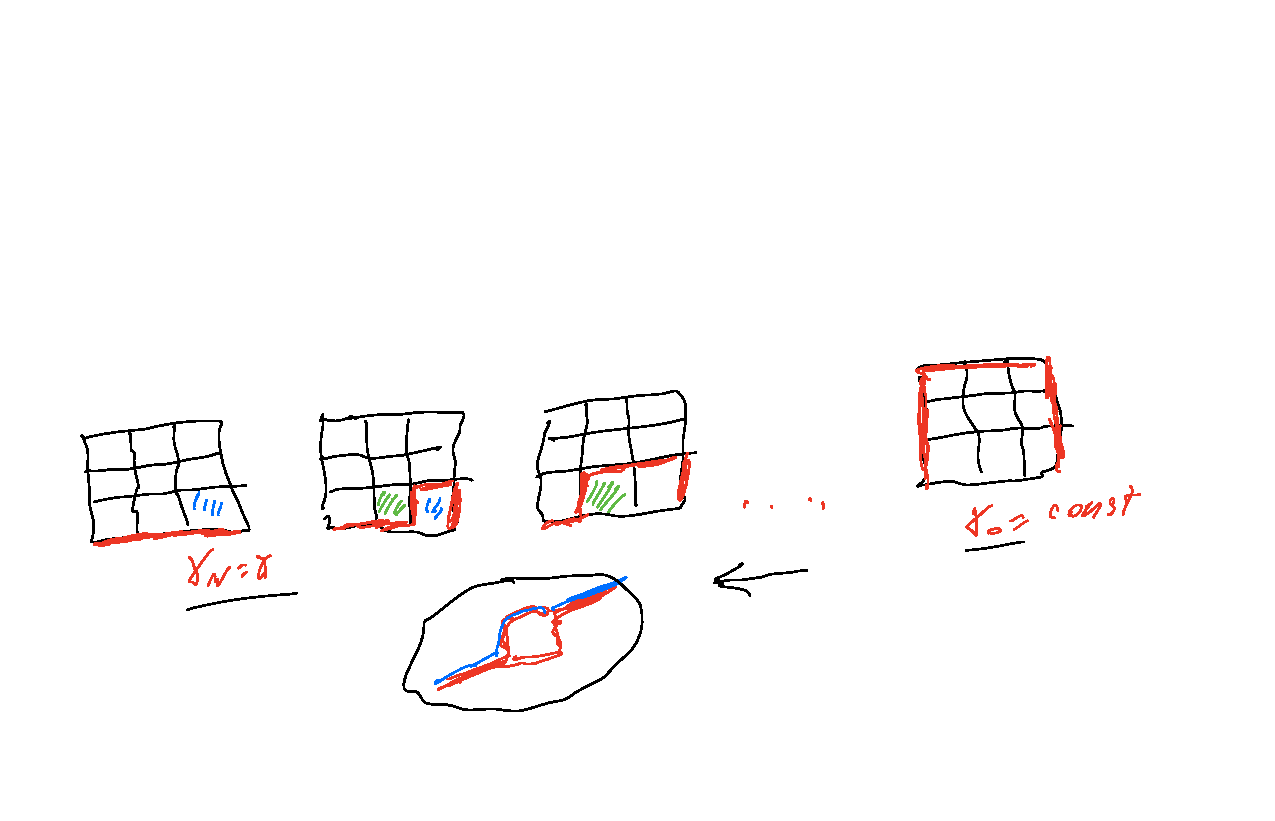
\includegraphics[height=5cm]{DG-01.pdf}
        \end{figure}

        Докажем, что в группе $\pi_1(Y, x_0)$ элементы $[\gamma_i]$ и $[\gamma_{i+1}]$ отличаются умножением на элемент из $N([\alpha])$. Запишем пути $\gamma_i$ и $\gamma_{i+1}$ в виде: $\gamma_i = uv_1w$, $\gamma_{i+1} = uv_2w$, где $u$, $v_1$, $v_2$, $w$ --- пути, $u$ и $w$ --- общие части $\gamma_i$ и $\gamma_{i+1}$, а $v_1$ и $v_2$ --- отличающиеся участки. Тогда $\gamma_{i+1} \sim u v_2 v_1^{-1} u^{-1} \gamma_i$. Т.е. $[\gamma_i]$ и $[\gamma_{i+1}]$ отличаются умножением на $[u v_2 v_1^{-1} u^{-1}]$. Всё классы гомотопности --- в пространстве $X \setminus \{q\}$.
        
        Осталось доказать, что $[u v_2 v_1^{-1} u^{-1}] \in N([\alpha])$. Обозначим $\beta = v_2v_1^{-1}$, в новых обозначениях надо доказать, что $[u\beta u^{-1}] \in N([\alpha])$. Петля $\beta$ --- образ границы маленького квадратика, а значит содержится и стягиваема либо в $X \setminus Y$, либо в $X \setminus \{q\}$.

        Если $\beta$ стягиваема в $X \setminus \{q\}$, то $u\beta u^{-1}$ тоже. Следовательно, $[u \beta u^{-1}]$ --- единица группы $\pi_1(X \setminus \{q\}, x_0)$, и тогда $[u \beta u^{-1}] \in N([\alpha])$.
        
        Если $\beta$ содержится в $X \setminus Y$, то она --- часть сетки, и поэтому не проходит через $q$. Подкруткой в диске и радиальной проекцией $\beta$ переводится в петлю $\beta_1 = \widehat{\alpha} \circ \theta$, где $\theta \in \Omega(S_1, (1, 0))$. Это реализуется гомотопией, определенной на всём $X \setminus \{q\}$; при этой гомотопии $u$ переходит в некоторую петлю $u_1 \in \Omega(Y, x_0)$. Значит петля $u \beta u^{-1}$ гомотопна произведению петель $u_1 \beta_1 u_1^{-1}$. Осталось доказать, что $[u_1 \beta_1 u_1^{-1}] \in N([\alpha])$. $\theta$ гомотопна $k$-кратному обходу окружности (для некоторого $k \in Z$). Следовательно, $\beta_1 \sim \alpha^k$. Тогда $[u_1 \beta_1 u_1^{-1}] = [u_1 \alpha^k u_1^{-1}] = [u_1 \alpha u_1^{-1}]^k \in N([\alpha])$.
    \end{proof}
    
    \begin{corollary}
        Если $\pi_1(Y) = \langle f_1, \dots, f_n \mid w_1(\overline{f}), \dots, w_k(\overline{f}) \rangle$, а $[\alpha] = w_{k+1}(\overline{f})$, то
        \[\pi_1(X) = \langle f_1, \dots, f_n \mid w_1(\overline{f}), \dots, w_{k+1}(\overline{f}) \rangle.\]
    \end{corollary}

    \begin{example}
        Тор --- это букет из двух окружностей, на которую наклеили 2-клетку. Поэтому фундаментальная группа тора --- $\langle a, b \mid a b a^{-1} b^{-1} \rangle = \ZZ^2.$
    \end{example}

    \begin{theorem}
        
    \end{theorem}

    % \subsection{Накрытия}
    % \subsection{Приложения}

    % \section{Дифференциальная геометрия}
    % \subsection{Гладкие кривые и поверхности}
    % \subsection{Гладкие многообразия}
    % \subsection{Римановы многообразия}

\end{document}